\begin{pastexam}[label={px:ncu-108-dsa-02}]{中央資工所 108 學年度 第 2 題}
（單選；每題 5 分，答錯倒扣 1 分）

Build a \textit{binary search tree} for the input sequence 9, 4, 8, 7, 20, 15, 14, 3, 10. It is
assumed that the tree root is on level 1.
\begin{enumerate}[label=(\Alph*)]
\item There are five levels in the tree.
\item 20 is on level 3.
\item 7 and 10 have the same father.
\item The left subtree of 20 has 1 node.
\item None of the above
\end{enumerate}
\end{pastexam}

\begin{pastsoln}
答案：(A)。

依序插入（資結書虛擬碼~9.6）：每個鍵從根往下比，小的往左、大的往右，走到空的位置就放下。
\begin{itemize}
\item $9$：根。
\item $4 < 9$：$9$ 的左子。 $8$：$< 9$ 往左、$> 4$ 往右，$4$ 的右子。 $7$：$< 9$、$> 4$、$< 8$，$8$ 的左子。
\item $20 > 9$：$9$ 的右子。 $15$：$> 9$、$< 20$，$20$ 的左子。 $14$：$> 9$、$< 20$、$< 15$，$15$ 的左子。
\item $3$：$< 9$、$< 4$，$4$ 的左子。 $10$：$> 9$、$< 20$、$< 15$、$< 14$，$14$ 的左子。
\end{itemize}
\begin{center}
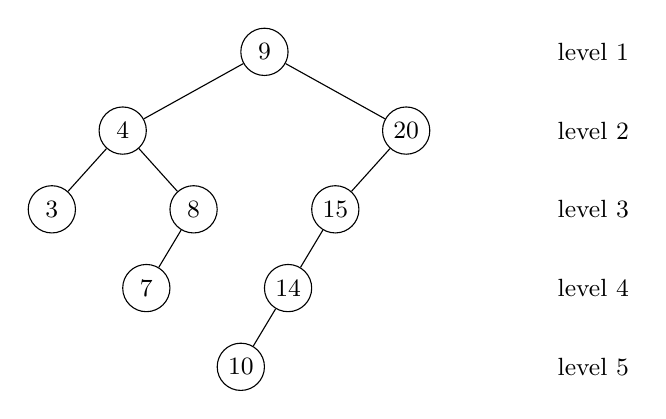
\begin{tikzpicture}[v/.style={circle,draw,inner sep=0pt,minimum size=6mm,font=\small},
  level distance=10mm, level 1/.style={sibling distance=36mm}, level 2/.style={sibling distance=18mm},
  level 3/.style={sibling distance=12mm}]
\node[v] {9}
  child {node[v] {4}
    child {node[v] {3}}
    child {node[v] {8} child {node[v] {7}} child[missing] {}}}
  child {node[v] {20}
    child {node[v] {15}
      child {node[v] {14} child {node[v] {10}} child[missing] {}}
      child[missing] {}}
    child[missing] {}};
\node[font=\small, anchor=west] at (3.6, 0) {level 1};
\node[font=\small, anchor=west] at (3.6, -1) {level 2};
\node[font=\small, anchor=west] at (3.6, -2) {level 3};
\node[font=\small, anchor=west] at (3.6, -3) {level 4};
\node[font=\small, anchor=west] at (3.6, -4) {level 5};
\end{tikzpicture}
\end{center}
各層：level 1 是 $9$；level 2 是 $4, 20$；level 3 是 $3, 8, 15$；level 4 是 $7, 14$；level 5 是 $10$。

逐項：
\begin{itemize}
\item (A) 五層：最深的 $10$ 在 level 5，對。
\item (B) $20$ 是根的右子，在 level 2，錯。
\item (C) $7$ 的父節點是 $8$，$10$ 的父節點是 $14$，錯。
\item (D) $20$ 的左子樹是 $15, 14, 10$ 三個節點，錯。
\item (E) (A) 對，所以錯。
\end{itemize}
\end{pastsoln}
